\documentclass{beamer}
\usepackage{animate}
\usepackage{amsmath}
\usepackage{tikz}
\usetheme{Madrid}
\usepackage{tikz}
\graphicspath{{./figures/}}
\setbeamercolor{structure}{fg=green!39!black} % changes main accent color to green

\useinnertheme{circles}

% Captions without the "Figure:" label (beamer prints the label by default).
\setbeamertemplate{caption}{\raggedright\insertcaption\par}
%Information to be included in the title page:
\title{Growing tissues and beyond}
\author{Jakub Koubele}
\institute{Beyer lab retreat}
\date{9th September, 2026}

\renewcommand{\insertshortauthor}{Jakub Koubele}  
\renewcommand{\insertshorttitle}{Growing tissues and beyond}
\renewcommand{\insertshortdate}{9th September, 2026} % Define custom text for 3rd block

\usepackage[authoryear]{natbib}
\bibliographystyle{apalike}
\usepackage{amsthm}
\newcommand*{\QED}{\hfill\ensuremath{\blacksquare}}
% Micrometres: thin space, upright unit. Use as \um{200}.
\newcommand{\um}[1]{\ensuremath{#1\,\mu\mathrm{m}}}
\setbeamertemplate{navigation symbols}{}





\begin{document}
	\frame{\titlepage}
	
	
	\begin{frame}
		\frametitle{Oxygen supply}	
			
	\centering
	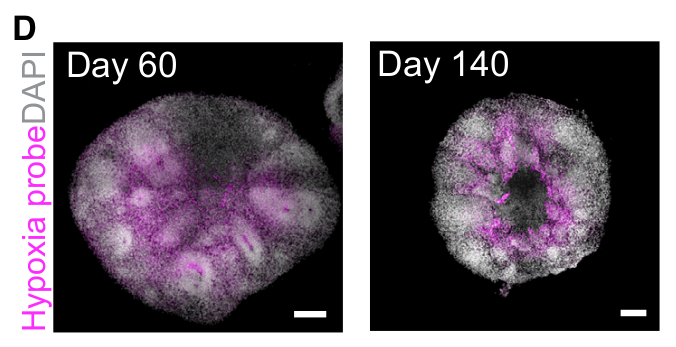
\includegraphics[width=10cm]{hypoxia_organoid}\\[0.4em]
	{\scriptsize Scale bar = \um{200}. Figure 1D from \citet{qianSlicedHumanCortical2020}. Note that day 140 is zoomed out, as the organoid grows over time.}
	
	\begin{itemize}
		\item Oxygen diffuses only up to \um{200} in tissues.
		\item A vascular system to deliver oxygen and nutrients is therefore necessary for tissue thicker than $\sim$~\um{400}.
	\end{itemize}		
		
	\end{frame}

	\begin{frame}
		\frametitle{Self-organization of cells}	
		\centering
		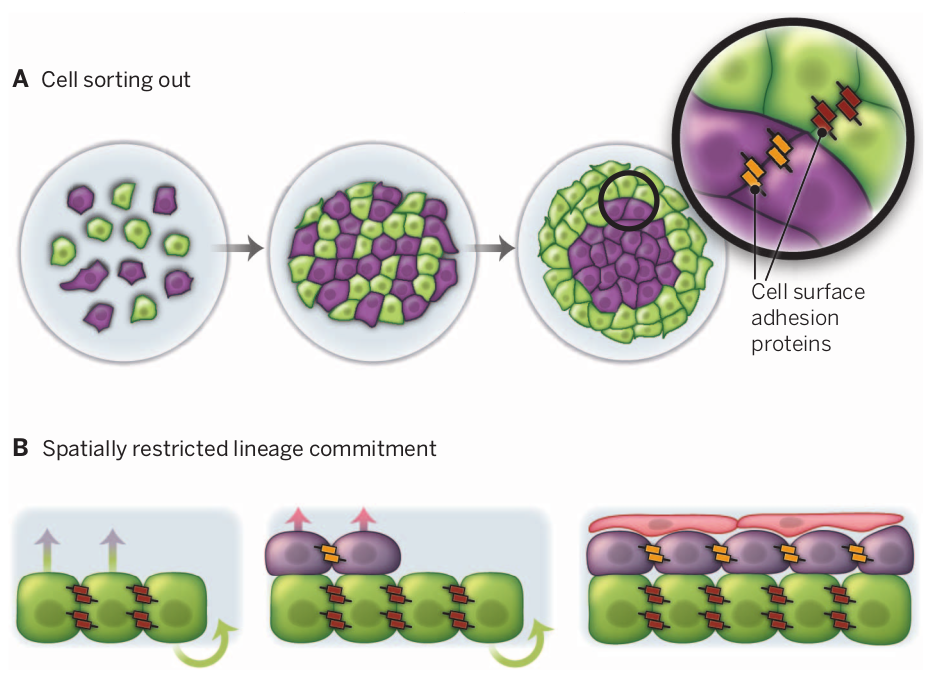
\includegraphics[width=7cm]{self_organization}\\[0.4em]
		{\scriptsize \textbf{Principles of self-organization}. Figure 2 from \citet{lancasterOrganogenesisDishModeling2014}.}

		\begin{itemize}
			\item Cells sort themselves by adhesion.			
			\item However, vessels require endothelial cells (a separate lineage).
			\item Active blood flow is also needed (vessels regress otherwise).
		\end{itemize}
	\end{frame}

\begin{frame}
	\frametitle{Vascularization of organoids}	
	\centering
	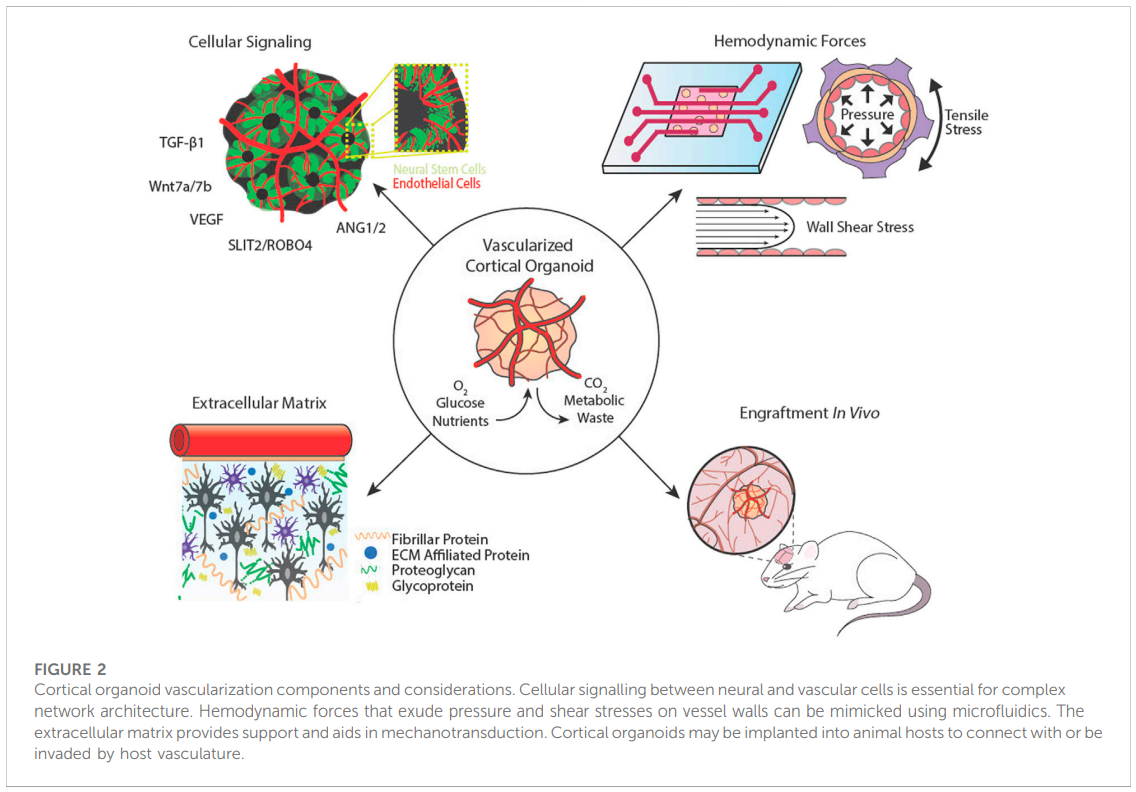
\includegraphics[width=10cm]{vascularized_organoid}\\[0.3em]
	{\scriptsize Figure 2 from \cite{lamontagneRecentAdvancementsFuture2022}.}
\end{frame}



\begin{frame}
	\frametitle{Vascularization of organoids (cont.)}	
	\centering
	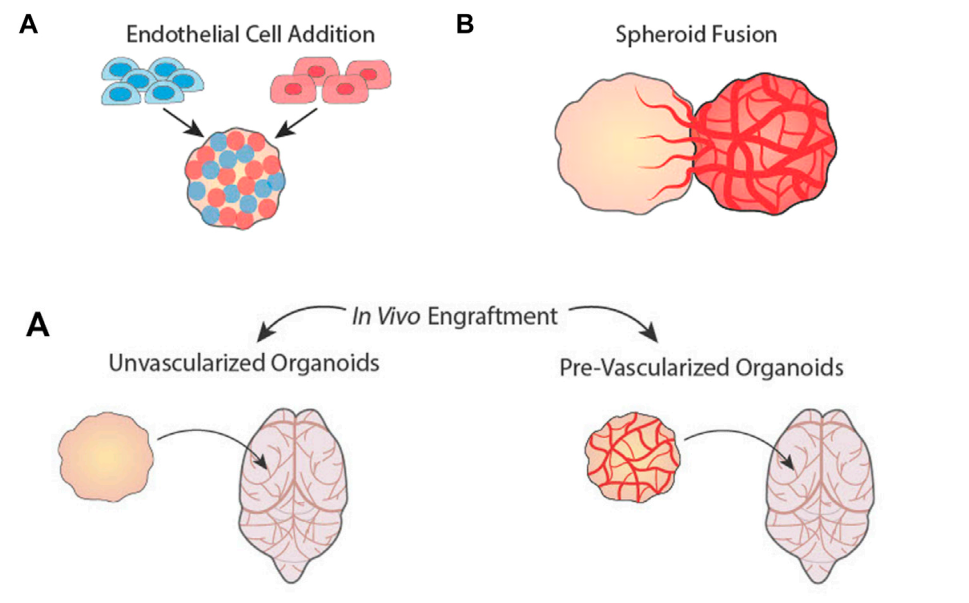
\includegraphics[width=10cm]{organoid_vasc_strategies}\\[0.3em]
	{\scriptsize Figures 3 and 5 from \cite{lamontagneRecentAdvancementsFuture2022}.}
\end{frame}


\begin{frame}
	\frametitle{Bioprinting}	
	\centering
	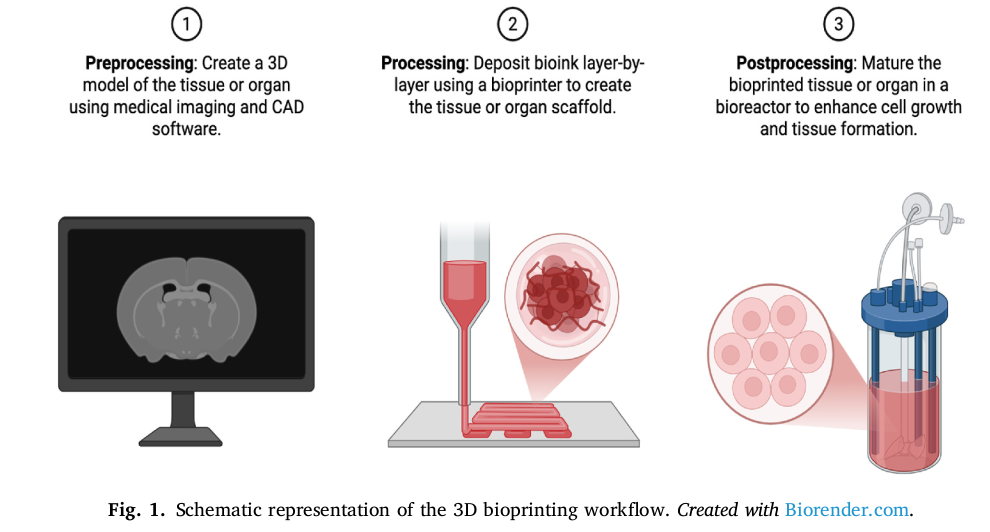
\includegraphics[width=8cm]{bioprinting}\\[0.3em]
	{\scriptsize Figure 1 from \citet{idnaniEngineeringFutureOrgan2026}.}
	
	\begin{itemize}
		\item 3D printing approach. Bioink = differentiated cells + ECM components.
		\item Need lots of cells (costly and challenging to produce). 
		\item Trade-offs between resolution, viscosity, speed and cell viability.
	\end{itemize}
\end{frame}

\begin{frame}
	\frametitle{Vascularization with bioprinting}
	\centering
	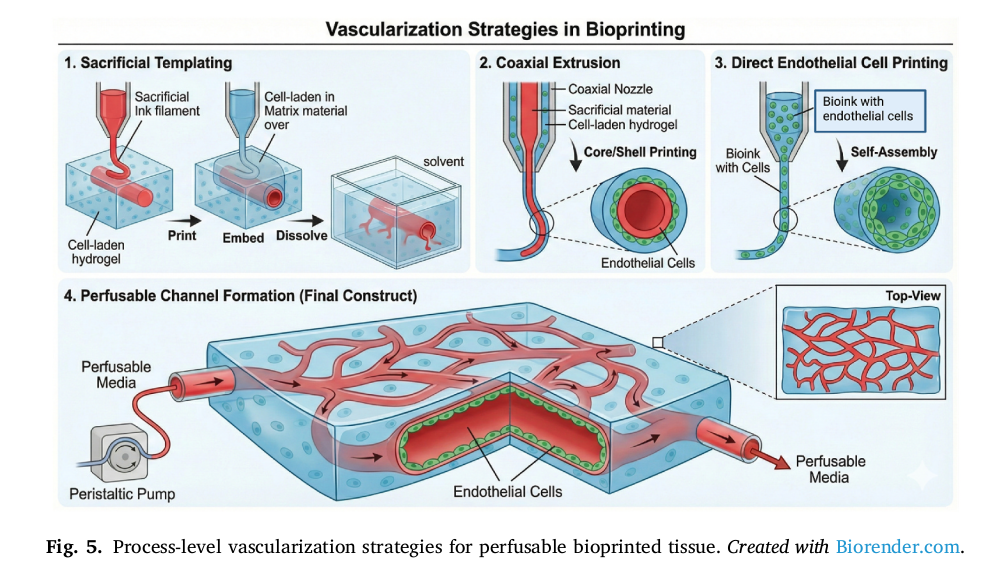
\includegraphics[width=8cm]{vasc_with_bioprint}\\[0.3em]
	{\scriptsize Figure 5 from \citet{idnaniEngineeringFutureOrgan2026}.}
	\begin{itemize}
		\item Bioprinting approaches help with vascularization, but the resolution is still far away from real capillaries.
	\end{itemize}
\end{frame}


\begin{frame}
	\frametitle{Decellularized matrix}
	\centering
	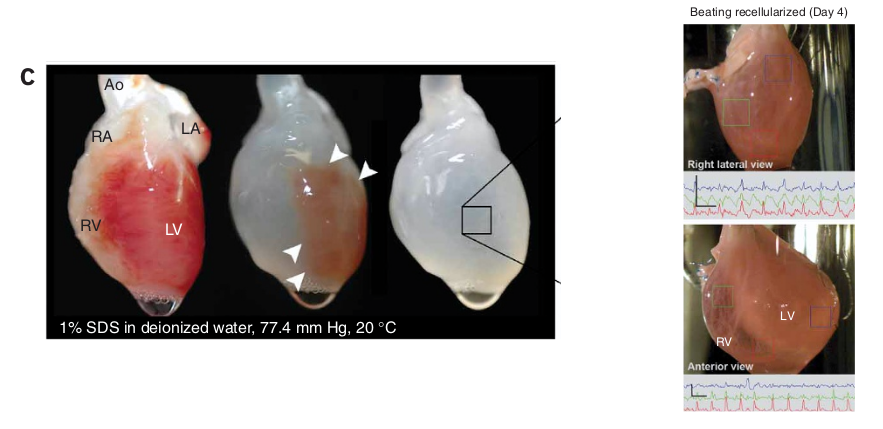
\includegraphics[width=8cm]{rat_heart}\\[0.3em]
	{\scriptsize Figures 1c and 4d from \citet{ottPerfusiondecellularizedMatrixUsing2008}.}
	
	\begin{itemize}
		\item Paper \textit{Perfusion-decellularized matrix: using nature’s platform to engineer a bioartificial heart}.
		\item Remove cells from a rat heart, keep the ECM. The vascular network is preserved.
		\item Repopulate with cells $\to$ it beats (but only $\sim$2\% of normal heart function).
	\end{itemize}
\end{frame}

\begin{frame}
	\frametitle{Engineered bladder}
	\centering
	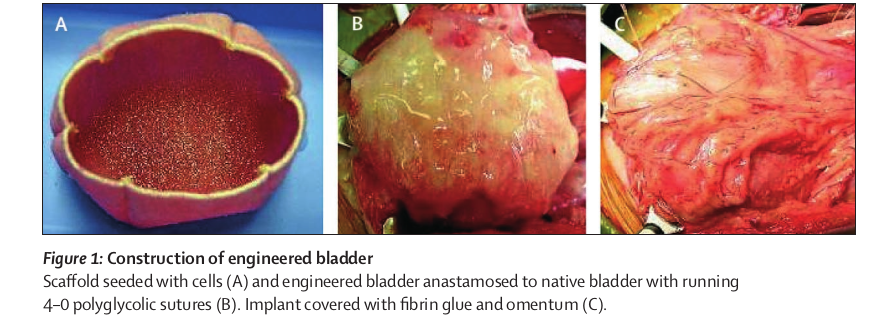
\includegraphics[width=11cm]{bladder}\\[0.3em]
	{\scriptsize Figure 1 from \citet{atalaTissueengineeredAutologousBladders2006}.}
	\begin{itemize}
		\item 2006: seven patients, their own bladder cells expanded onto a collagen-PGA scaffold.
		\item The host grows the blood supply into it. Worked because a bladder is thin, hollow and metabolically cheap.
	\end{itemize}
\end{frame}

\begin{frame}
	\frametitle{Trachea scandal}
	\centering
	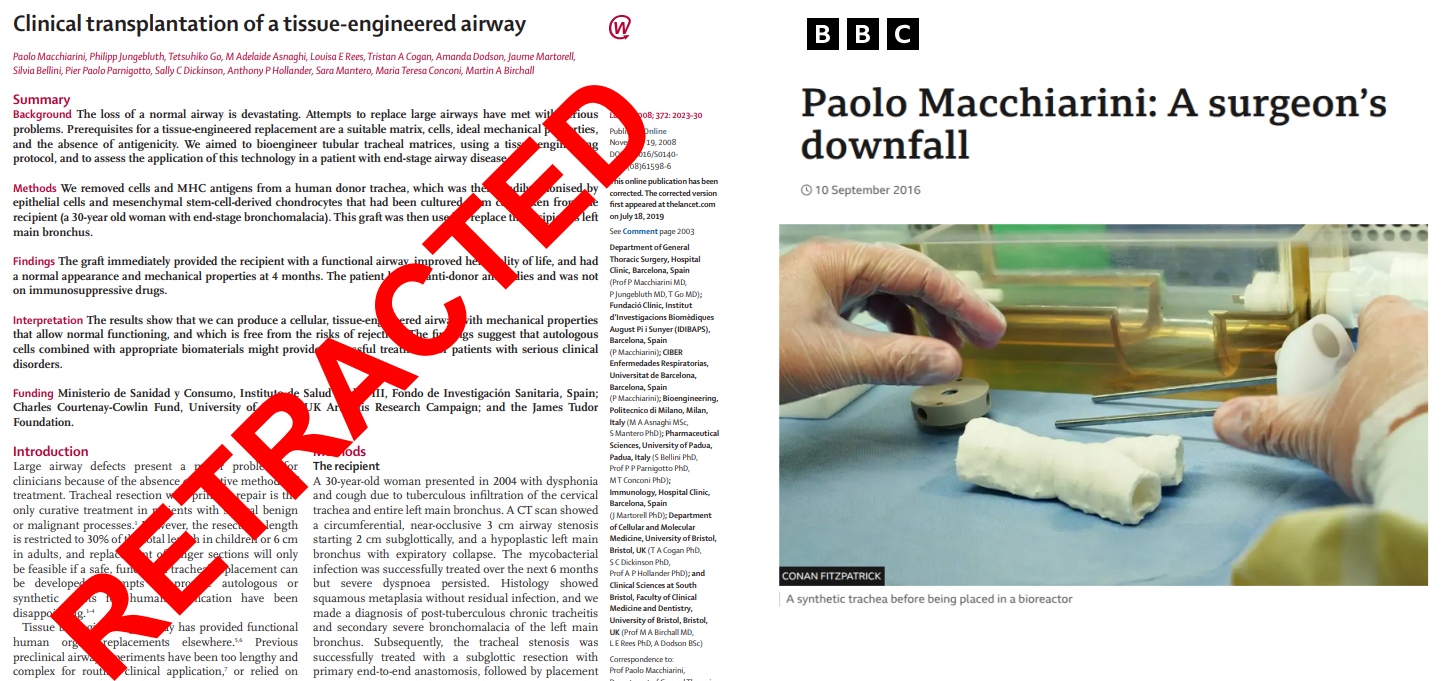
\includegraphics[width=10cm]{trachea}\\[0.3em]
	\begin{itemize}
		\item 2008--2013: tracheas (decellularized, later synthetic) seeded with the patients' own cells. Most recipients died.
		\item No blood supply --- a trachea has no single artery, just many small vessels.
		\item Four \textit{Lancet} papers retracted; Macchiarini convicted of gross assault in Sweden (2023).
	\end{itemize}
\end{frame}

\begin{frame}
	\frametitle{Synthetic embryos}
	\centering
	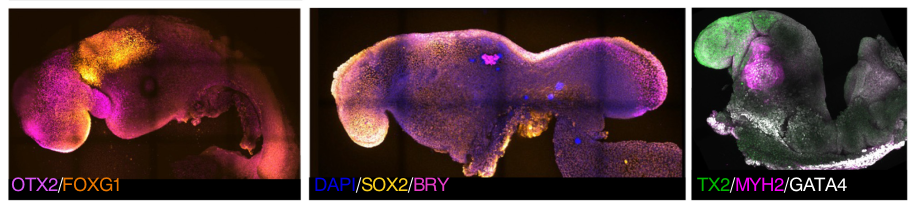
\includegraphics[width=10cm]{embryos}\\[0.3em]
	{\scriptsize Mouse embryo models can develop to the organogenesis stage. Figure 5C from \citet{fuUnlockingPotentialStemcellderived2025}.}
	\begin{itemize}
		\item Built from stem cells alone (no egg/sperm).
		\item Reach only E8.5 --- neural tube, gut and beating heart (even natural embryos stop at E11 in a dish).
		\item Dies without a placenta to connect to (engineered placentas for embryos do not exist yet).
	\end{itemize}
	
\end{frame}


\begin{frame}
	\frametitle{The end}
	\centering
	Thank you for the attention!\\[0.7em]
	\centering
	
\includegraphics[width=10cm]{group_picture}\\[0.3em]
\end{frame}


\begin{frame}
	\frametitle{References}
	{\scriptsize
	\bibliography{../references}}
\end{frame}
	
	

	
	
\end{document}
